\documentclass[12pt, xcolor=table]{beamer}
\usepackage{graphicx}
\usepackage[ngerman]{babel}
\usepackage[utf8]{inputenc}
\usepackage{amsmath}
\usepackage{amssymb}
\usepackage{listings}
\usepackage{hyperref}
\usepackage{fancyvrb}
\usepackage{color}
\usepackage{verbatim}

\usepackage[percent]{overpic}
\usepackage[footnotesize, bf]{caption}
%Copyright 2008 by Adrian Böhmichen
%
% This file is free software: you can redistribute it and/or modify
% it under the terms of the GNU General Public License as published by
% the Free Software Foundation, either version 3 of the License, or
% (at your option) any later version.
%
% This file is distributed in the hope that it will be useful,
% but WITHOUT ANY WARRANTY; without even the implied warranty of
% MERCHANTABILITY or FITNESS FOR A PARTICULAR PURPOSE.  See the
% GNU General Public License for more details.
%
% You should have received a copy of the GNU General Public License
% along with this file.  If not, see <http://www.gnu.org/licenses/>.

%%%%%%%%%%%%%%%%%%%%%%%%%%%%%%%%%%%%%%%%%%%%%%%%%%%%%%%%%%%%%%%%%
%     Ubuntuusers Vorlage für ein LaTeX-Beamer Theme            %
%                                                               %
% Für das Korrekte funktionieren benötigt man einen header.png  %
% und ein logo.png Datei!                                       %
% Zusätzlich muss man folgende Pakete benutzten:                %
%   \usepackage{graphicx}                                       %
%   \usepackage[percent]{overpic}                               %
%                                                               %
% Danach muss nur noch am Anfang die Datei                      %
% mit \input{} eingebunden werden.                              %
%                                                               %
%%%%%%%%%%%%%%%%%%%%%%%%%%%%%%%%%%%%%%%%%%%%%%%%%%%%%%%%%%%%%%%%%

%weitere Farbe spezifizieren:
%Farben von dem Humantheme
%\definecolor{Orange}{RGB}{240,165,19}
\definecolor{Orange}{RGB}{5,215,242}
%\definecolor{Human-Base}{RGB}{129,102,71}
\definecolor{Human-Base}{RGB}{5,25,242}
%Farben aus dem Inyokatheme
%\definecolor{uuheader1}{RGB}{164,143,101}
\definecolor{uuheader1}{RGB}{5,25,242}
%\definecolor{uuheader2}{RGB}{129,106,59}
\definecolor{uuheader2}{RGB}{5,25,242}


%Theme festlegen für alle Templates die nicht selbstständig definiert werden:
\usepackage{beamerthemedefault}


%Definieren des Innertheme, zuständig für die Symbole bei Listen
\setbeamertemplate{sections/subsections in toc}[circle]
\setbeamertemplate{items}[circle]

\setbeamercolor{item}{fg=Human-Base}

%entfernen der Navigationsleiste
\beamertemplatenavigationsymbolsempty

%Logo definieren, man kann die Lage nicht verändern
%\logo{\includegraphics[scale=0.1]{logo.png}}


%Kopf- und Fußzeile definieren
%\setbeamertemplate{headline}
%{%
%\begin{overpic}[width=\paperwidth
% nächste Zeile dient zum anzeigen eines Rasters, für das paltzieren des ToC hilfreich
%,grid,tics=10
%]
%{header.png}%
%  \put(0,11){\insertsectionnavigationhorizontal{\paperwidth}{~}{~}}%
%  \end{overpic}
%}

\setbeamertemplate{footline}[text line]
{%
\begin{minipage}[b]{116mm}
\insertauthor \hfill%
%neue Navigationsleiste
 \insertframenumber ~/ \inserttotalframenumber\\[1ex]
\end{minipage}
}

% Farben festlegen ausserhalb des innertheme

%Allgemeine Angaben und Verbesserung vom default Theme
\setbeamercolor{structure}{fg=uuheader1}
\setbeamercolor{section in toc}{fg=Human-Base}
\setbeamercolor{subsection in toc}{parent=section in toc}
\setbeamercolor{framesubtitle}{fg=uuheader2}


%Farbe und Form der Blöcke definieren
\setbeamertemplate{blocks}[rounded]
%\setbeamercolor{block title}{fg=uuheader1,bg=Orange}
%\setbeamercolor{block title alerted}{use=alerted text,fg=black,bg=alerted text.fg!75!bg}
%\setbeamercolor{block title example}{use=example text,fg=black,bg=example text.fg!75!bg}

%\setbeamercolor{block body}{parent=normal text,use=block title,bg=block title.bg!25!bg}
%\setbeamercolor{block body alerted}{parent=normal text,use=block title alerted,bg=block title alerted.bg!25!bg}
%\setbeamercolor{block body example}{parent=normal text,use=block title example,bg=block title example.bg!25!bg}

%Für den Titleframe
\setbeamertemplate{title page}[default][rounded=true]
\setbeamercolor{title}{fg=uuheader2}
%,bg=Orange}


\makeatletter
\def\PY@reset{\let\PY@it=\relax \let\PY@bf=\relax%
    \let\PY@ul=\relax \let\PY@tc=\relax%
    \let\PY@bc=\relax \let\PY@ff=\relax}
\def\PY@tok#1{\csname PY@tok@#1\endcsname}
\def\PY@toks#1+{\ifx\relax#1\empty\else%
    \PY@tok{#1}\expandafter\PY@toks\fi}
\def\PY@do#1{\PY@bc{\PY@tc{\PY@ul{%
    \PY@it{\PY@bf{\PY@ff{#1}}}}}}}
\def\PY#1#2{\PY@reset\PY@toks#1+\relax+\PY@do{#2}}

\def\PY@tok@gd{\def\PY@tc##1{\textcolor[rgb]{0.63,0.00,0.00}{##1}}}
\def\PY@tok@gu{\let\PY@bf=\textbf\def\PY@tc##1{\textcolor[rgb]{0.50,0.00,0.50}{##1}}}
\def\PY@tok@gt{\def\PY@tc##1{\textcolor[rgb]{0.00,0.25,0.82}{##1}}}
\def\PY@tok@gs{\let\PY@bf=\textbf}
\def\PY@tok@gr{\def\PY@tc##1{\textcolor[rgb]{1.00,0.00,0.00}{##1}}}
\def\PY@tok@cm{\let\PY@it=\textit\def\PY@tc##1{\textcolor[rgb]{0.25,0.50,0.50}{##1}}}
\def\PY@tok@vg{\def\PY@tc##1{\textcolor[rgb]{0.10,0.09,0.49}{##1}}}
\def\PY@tok@m{\def\PY@tc##1{\textcolor[rgb]{0.40,0.40,0.40}{##1}}}
\def\PY@tok@mh{\def\PY@tc##1{\textcolor[rgb]{0.40,0.40,0.40}{##1}}}
\def\PY@tok@go{\def\PY@tc##1{\textcolor[rgb]{0.50,0.50,0.50}{##1}}}
\def\PY@tok@ge{\let\PY@it=\textit}
\def\PY@tok@vc{\def\PY@tc##1{\textcolor[rgb]{0.10,0.09,0.49}{##1}}}
\def\PY@tok@il{\def\PY@tc##1{\textcolor[rgb]{0.40,0.40,0.40}{##1}}}
\def\PY@tok@cs{\let\PY@it=\textit\def\PY@tc##1{\textcolor[rgb]{0.25,0.50,0.50}{##1}}}
\def\PY@tok@cp{\def\PY@tc##1{\textcolor[rgb]{0.74,0.48,0.00}{##1}}}
\def\PY@tok@gi{\def\PY@tc##1{\textcolor[rgb]{0.00,0.63,0.00}{##1}}}
\def\PY@tok@gh{\let\PY@bf=\textbf\def\PY@tc##1{\textcolor[rgb]{0.00,0.00,0.50}{##1}}}
\def\PY@tok@ni{\let\PY@bf=\textbf\def\PY@tc##1{\textcolor[rgb]{0.60,0.60,0.60}{##1}}}
\def\PY@tok@nl{\def\PY@tc##1{\textcolor[rgb]{0.63,0.63,0.00}{##1}}}
\def\PY@tok@nn{\let\PY@bf=\textbf\def\PY@tc##1{\textcolor[rgb]{0.00,0.00,1.00}{##1}}}
\def\PY@tok@no{\def\PY@tc##1{\textcolor[rgb]{0.53,0.00,0.00}{##1}}}
\def\PY@tok@na{\def\PY@tc##1{\textcolor[rgb]{0.49,0.56,0.16}{##1}}}
\def\PY@tok@nb{\def\PY@tc##1{\textcolor[rgb]{0.00,0.50,0.00}{##1}}}
\def\PY@tok@nc{\let\PY@bf=\textbf\def\PY@tc##1{\textcolor[rgb]{0.00,0.00,1.00}{##1}}}
\def\PY@tok@nd{\def\PY@tc##1{\textcolor[rgb]{0.67,0.13,1.00}{##1}}}
\def\PY@tok@ne{\let\PY@bf=\textbf\def\PY@tc##1{\textcolor[rgb]{0.82,0.25,0.23}{##1}}}
\def\PY@tok@nf{\def\PY@tc##1{\textcolor[rgb]{0.00,0.00,1.00}{##1}}}
\def\PY@tok@si{\let\PY@bf=\textbf\def\PY@tc##1{\textcolor[rgb]{0.73,0.40,0.53}{##1}}}
\def\PY@tok@s2{\def\PY@tc##1{\textcolor[rgb]{0.73,0.13,0.13}{##1}}}
\def\PY@tok@vi{\def\PY@tc##1{\textcolor[rgb]{0.10,0.09,0.49}{##1}}}
\def\PY@tok@nt{\let\PY@bf=\textbf\def\PY@tc##1{\textcolor[rgb]{0.00,0.50,0.00}{##1}}}
\def\PY@tok@nv{\def\PY@tc##1{\textcolor[rgb]{0.10,0.09,0.49}{##1}}}
\def\PY@tok@s1{\def\PY@tc##1{\textcolor[rgb]{0.73,0.13,0.13}{##1}}}
\def\PY@tok@sh{\def\PY@tc##1{\textcolor[rgb]{0.73,0.13,0.13}{##1}}}
\def\PY@tok@sc{\def\PY@tc##1{\textcolor[rgb]{0.73,0.13,0.13}{##1}}}
\def\PY@tok@sx{\def\PY@tc##1{\textcolor[rgb]{0.00,0.50,0.00}{##1}}}
\def\PY@tok@bp{\def\PY@tc##1{\textcolor[rgb]{0.00,0.50,0.00}{##1}}}
\def\PY@tok@c1{\let\PY@it=\textit\def\PY@tc##1{\textcolor[rgb]{0.25,0.50,0.50}{##1}}}
\def\PY@tok@kc{\let\PY@bf=\textbf\def\PY@tc##1{\textcolor[rgb]{0.00,0.50,0.00}{##1}}}
\def\PY@tok@c{\let\PY@it=\textit\def\PY@tc##1{\textcolor[rgb]{0.25,0.50,0.50}{##1}}}
\def\PY@tok@mf{\def\PY@tc##1{\textcolor[rgb]{0.40,0.40,0.40}{##1}}}
\def\PY@tok@err{\def\PY@bc##1{\fcolorbox[rgb]{1.00,0.00,0.00}{1,1,1}{##1}}}
\def\PY@tok@kd{\let\PY@bf=\textbf\def\PY@tc##1{\textcolor[rgb]{0.00,0.50,0.00}{##1}}}
\def\PY@tok@ss{\def\PY@tc##1{\textcolor[rgb]{0.10,0.09,0.49}{##1}}}
\def\PY@tok@sr{\def\PY@tc##1{\textcolor[rgb]{0.73,0.40,0.53}{##1}}}
\def\PY@tok@mo{\def\PY@tc##1{\textcolor[rgb]{0.40,0.40,0.40}{##1}}}
\def\PY@tok@kn{\let\PY@bf=\textbf\def\PY@tc##1{\textcolor[rgb]{0.00,0.50,0.00}{##1}}}
\def\PY@tok@mi{\def\PY@tc##1{\textcolor[rgb]{0.40,0.40,0.40}{##1}}}
\def\PY@tok@gp{\let\PY@bf=\textbf\def\PY@tc##1{\textcolor[rgb]{0.00,0.00,0.50}{##1}}}
\def\PY@tok@o{\def\PY@tc##1{\textcolor[rgb]{0.40,0.40,0.40}{##1}}}
\def\PY@tok@kr{\let\PY@bf=\textbf\def\PY@tc##1{\textcolor[rgb]{0.00,0.50,0.00}{##1}}}
\def\PY@tok@s{\def\PY@tc##1{\textcolor[rgb]{0.73,0.13,0.13}{##1}}}
\def\PY@tok@kp{\def\PY@tc##1{\textcolor[rgb]{0.00,0.50,0.00}{##1}}}
\def\PY@tok@w{\def\PY@tc##1{\textcolor[rgb]{0.73,0.73,0.73}{##1}}}
\def\PY@tok@kt{\def\PY@tc##1{\textcolor[rgb]{0.69,0.00,0.25}{##1}}}
\def\PY@tok@ow{\let\PY@bf=\textbf\def\PY@tc##1{\textcolor[rgb]{0.67,0.13,1.00}{##1}}}
\def\PY@tok@sb{\def\PY@tc##1{\textcolor[rgb]{0.73,0.13,0.13}{##1}}}
\def\PY@tok@k{\let\PY@bf=\textbf\def\PY@tc##1{\textcolor[rgb]{0.00,0.50,0.00}{##1}}}
\def\PY@tok@se{\let\PY@bf=\textbf\def\PY@tc##1{\textcolor[rgb]{0.73,0.40,0.13}{##1}}}
\def\PY@tok@sd{\let\PY@it=\textit\def\PY@tc##1{\textcolor[rgb]{0.73,0.13,0.13}{##1}}}

\def\PYZbs{\char`\\}
\def\PYZus{\char`\_}
\def\PYZob{\char`\{}
\def\PYZcb{\char`\}}
\def\PYZca{\char`\^}
\def\PYZsh{\char`\#}
\def\PYZpc{\char`\%}
\def\PYZdl{\char`\$}
\def\PYZti{\char`\~}
% for compatibility with earlier versions
\def\PYZat{@}
\def\PYZlb{[}
\def\PYZrb{]}
\makeatother

\renewcommand{\footnotesize}{\tiny}

\begin{document}
\title{Endpräsentation - Multilabel Classification}
\author{peterr und Lusy}
\date{\today}

\begin{frame}
    \titlepage
    \begin{block}
        \tiny \url{https://github.com/lusy/multilabel\_classification}
    \end{block}
\end{frame}

\begin{frame}
    \frametitle{Übersicht}
    \tableofcontents
\end{frame}

\begin{frame}
     \frametitle{Einleitung}
     \begin{itemize}
         \item Reduktion der Features durch Topic Models
         \item Multilabel problem, jeder Eintrag  kann in mehreren Klassen fallen
     \end{itemize}
\end{frame}

\section{Datensatz}
\begin{frame}
    \frametitle{Datensatz}
    \begin{itemize}
        \item mathematische Publikationen mit Titeln und Abstracts
        \item enthält  $1.1$ Mio. Dokumente
        \item jedes Dokument hat min. 1 Label
        \item $75.6 \%$ 1 Label, $24.3 \%$ 2 Label und ca. $0.1 \%$ mehr Labels
    %\item aus welchen Jahren sind die Publikationen
    \end{itemize}
    \begin{block}{Auszug}
        \begin{table}
            \rowcolors[]{1}{blue!20}{blue!10}
            \begin{tabular}{cccll}
                \tiny\textbf{ID} &\tiny \textbf{CLASSES} &\tiny \textbf{YEAR} &\tiny \textbf{TITLE} & \tiny \textbf{ABSTRACT} \\
                \hline
                \tiny 1000000796 &\tiny EW & \tiny 2000 & \tiny Dynamo: A transparent dynamic \dots  & \tiny We describe the design \dots \\
                \tiny 1000000815 &\tiny EW & \tiny 2000 & \tiny Unification-based pointer \dots  & \tiny This paper describes \dots \\
                \multicolumn{5}{c}{\dots} \\
                \tiny 1000003814 &\tiny EV,PE & \tiny 1995 & \tiny A GENETIC APPROACH TO \dots  & \tiny The quadratic assignment \dots \\
                \tiny 1000004333 & \tiny PQ,EX &\tiny 1995 &\tiny DYNAMIC EUCLIDEAN MINIMUM \dots & \tiny We maintain the minimum \dots \\
            \end{tabular}
             \caption*{Auszug des Datensatzes}
        \end{table}
    \end{block}
\end{frame}

\subsection{Idee} % (fold)
\begin{frame}
     \frametitle{Idee}
     \begin{itemize}
         \item jeder Eintrag hat mehrere Labels
         \item State-of-the-Art Textklassifikation mit SVM und Text im Vector-Space-Model
         \item Nachteil: sehr großer Featureraum - jedes Wort ist Feature
         \item Ansatz: Featurereduktion mit Topic Models
     \end{itemize}
\end{frame}

\section{Tools}
\begin{frame}
    \frametitle{Tools}
    \begin{itemize}
        \item Vorverabeitung: bash, python (+scipy, scikit-learn)
        \item SVM: scikit-learn (LinearSVC)
        \item LDA: mallet
    \end{itemize}
\end{frame}

\section{Vorbereitung SVM}
\begin{frame}
    \frametitle{Vorbereitung SVM}
    \begin{itemize}
        \item Darstellung der Texte im Vector-space-model
        \item entfernen von Stopwörtern(is, and, the, \ldots)
        \item Vokabular mit $n$ Wörtern: alle vorkommende Wörter in den Texten
    \end{itemize}
        \begin{table}
            \rowcolors[]{1}{blue!20}{blue!10}
            \begin{tabular}{c|cccc}
                \tiny\textbf{$doc_{id}$} &\tiny \textbf{$word_{1}$} &\tiny \textbf{$word_{2}$} &\tiny \textbf{\dots} & \tiny \textbf{$word_{n}$} \\
                \hline
                \tiny 1000000796 &\tiny 1 & \tiny 2 & \tiny  \dots  & \tiny 0 \\
                \tiny 1000000815 &\tiny 0 & \tiny 3 & \tiny \dots  & \tiny 1 \\
                \multicolumn{5}{c}{\dots} \\
                \tiny 1000003814 &\tiny 2  & \tiny 0 & \tiny  \dots  & \tiny 0 \\
                \tiny 1000004333 & \tiny 0 &\tiny 0 &\tiny  \dots & \tiny 1 \\
            \end{tabular}
             \caption*{Darstellung im Vektor space model}
        \end{table}
\end{frame}
\section{Topic Models mit LDA}
\begin{frame}
    \frametitle{Topic models mit LDA}
    \begin{center}
        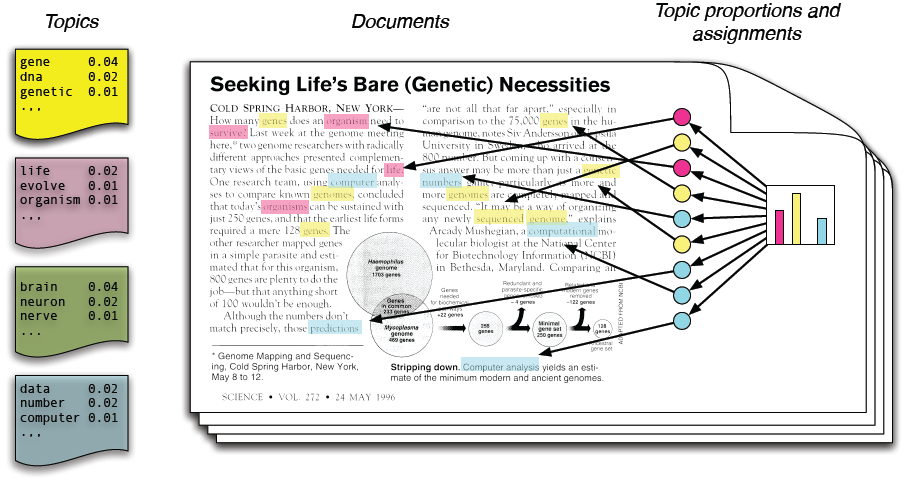
\includegraphics[scale=0.35]{figures/IntroToLDA.png}
    \end{center}
\end{frame}

\section{Vorbereitung Topic Models}
\begin{frame}
    \frametitle{Vorbereitung Topic models}
    \begin{itemize}
        \item Verteilung der Topics ist Feature für Dokumente
        \item Werte zwischen 0 und 1
        \item Summe für Einträge eines Dokuments beträgt 1
        \item Eintrag i enthält die Wahrscheinlichkeit für Topic i
        \item $\#topics << \#words$
    \end{itemize}
        \begin{table}
            \rowcolors[]{1}{blue!20}{blue!10}
            \begin{tabular}{c|cccc}
                \tiny\textbf{$doc_{id}$} &\tiny \textbf{$topic_{1}$} &\tiny \textbf{$topic_{2}$} &\tiny \textbf{\dots} & \tiny \textbf{$topic_{n}$} \\
                \hline
                \tiny 1000000796 &\tiny 0.1 & \tiny 0.05 & \tiny  \dots  & \tiny $1 \cdot 10^{-6}$  \\
                \tiny 1000000815 &\tiny 0.0 & \tiny 0.2 & \tiny \dots  & \tiny 0.1 \\
                \multicolumn{5}{c}{\dots} \\
                \tiny 1000003814 &\tiny 0.3  & \tiny $1 \cdot 10^{-6}$ & \tiny  \dots  & \tiny 0.0 \\
                \tiny 1000004333 & \tiny 0.0 &\tiny 0.0 &\tiny  \dots & \tiny 0.2 \\
            \end{tabular}
            \caption*{Repräsentation durch Topic Verteilung}
        \end{table}
\end{frame}
\end{frame}

\section{Sampling der Daten}
\begin{frame}
    \frametitle{Sampling der Daten}
    \begin{itemize}
        \item Stratified Sampling
        \item anhand der Labelkombinationen, also 'EW,PE' eine Klasse
        \item jedes Label kommt sowohl in Testdatensatz und Trainingsdatensatz vor
        \item Aufteilung: 70\% zum Trainieren und 30 \% zum Testen
    \end{itemize}
\end{frame}

\section{Ergebnisse der SVM}
\begin{frame}
    \frametitle{Ergebnisse der SVM}
\end{frame}
\subsection{Labelkombinationen} % (fold)
\begin{frame}
    \frametitle{Labelkombinationen}
\end{frame}

\subsection{Multilabel} % (fold)
\begin{frame}
    \frametitle{Multilabel}
\end{frame}

\section{Ergebnisse mit Topic Models}
\begin{frame}
    \frametitle{Datensatz}
\end{frame}
\subsection{Labelkombinationen} % (fold)
\begin{frame}
     \frametitle{Labelkombinationen}
\end{frame}

\subsection{Multilabel} % (fold)
\begin{frame}
     \frametitle{Multilabel}
\end{frame}

\section{Ursachen und Probleme}
\begin{frame}
    \frametitle{Probleme}
    \begin{itemize}
        \item Wahrscheinlichkeiten der Topics sehr schnell sehr klein
        \item Vektoren sind voll besetzt im Gegensatz zu unigram-Modell
        \item großer Speicheraufwand
        \item Ansatz performt nicht auf ungesehen Daten
    \end{itemize}
\end{frame}

\section{Ausblick} % (fold)
\begin{frame}
    \frametitle{Ausblick}
    \begin{itemize}
        \item keinen
    \end{itemize}
\end{frame}


\end{document}
